\documentclass[12pt,a4paper]{article}

\usepackage[T1]{fontenc}
\usepackage[utf8]{inputenc} % Use UTF-8 encoding for input
\usepackage{babel} 
\babelprovide[import=fr, main]{french} % Set the document language to French
       
\usepackage{lmodern}			       
\usepackage{amsmath}
\usepackage{amsfonts}
\usepackage{amssymb}
\usepackage{graphicx}
\usepackage{xcolor}
\usepackage{mathtools}
\usepackage{fancyhdr}
\usepackage{enumitem}
\usepackage{tcolorbox}
\usepackage{stmaryrd}
\usepackage[linesnumbered,ruled,vlined]{algorithm2e}
\usepackage[text={15cm,24.5cm},centering]{geometry}




\begin{document}


\begin{figure}[t]
    \centering
    
\includegraphics[width=5cm]{src/inp_n7.png}
    \hfill
    
\includegraphics[width=3.8cm]{src/insa_toulouse.png}
\end{figure}

\begin{center}
    \textbf{\LARGE Analyse des phénomènes dispersifs et application à la modélisation
    fluviale}
\end{center}

\vspace{0.5cm}

\begin{center}
    \text{Félix Foucher de Brandois}
\end{center}


\section*{Introduction}
On souhaite étudier dans ce projet le comportement d’un produit déversé dans une rivière de largeur constante $b$ et animée d’une vitesse $V$.
Ce produit est supposé peu miscible à l’eau et moins dense que l’eau (par exemple de l’huile), de sorte qu’il flotte à la surface de l’eau.


\section*{Mise en équation}
\begin{enumerate}
    \item On commence par mettre en équation le problème physique. On a les équations suivantes :
    \begin{itemize}
        \item Conservation de la masse : $\frac{\partial \rho}{\partial t} + \text{div}(\rho V) = 0$
        \item Conservation de la concentration : $\frac{\partial \rho C}{\partial t} + \text{div}(\Phi) = 0$
        \item Expression du flux : $\Phi = -\lambda \nabla C + \rho C V$
    \end{itemize}
    
    \begin{align*}
        \text{On a donc :} \quad & \frac{\partial \rho C}{\partial t} + \text{div}(-\lambda \nabla C + \rho C V) = 0 \\
        \Leftrightarrow \quad & \rho \frac{\partial C}{\partial t} + C \frac{\partial \rho}{\partial t} - \lambda \Delta C + C \text{div}(\rho V) + \rho V \nabla C = 0 \\
        \Leftrightarrow \quad & \rho \frac{\partial C}{\partial t} - C \text{div}(\rho V) - \lambda \Delta C + C \text{div}(\rho V) + \rho V \nabla C = 0 \\
        \Leftrightarrow \quad & \frac{\partial C}{\partial t} - \frac{\lambda}{\rho} \Delta C + V \nabla C = 0
    \end{align*}

\end{enumerate}

\section*{Approximation spatiale du Laplacien}
\begin{enumerate}[resume]

    \item On cherche maintenant à discrétiser le problème. Cela nécessite d'approximer le Laplacien de $u$.
    On utilise un développement de Taylor à l'ordre 3 de $u(x_{i+1}, y_j)$ et de $u(x_{i-1}, y_j)$ :
    \begin{align*}
        u(x_{i+1}, y_j) &= u(x_i, y_j) + h_x \frac{\partial u}{\partial x}(x_i, y_j) + \frac{h_x^2}{2} \frac{\partial^2 u}{\partial x^2}(x_i, y_j) + \frac{h_x^3}{6} \frac{\partial^3 u}{\partial x^3}(x_i, y_j) + \mathcal{O}(h_x^4) \\
        u(x_{i-1}, y_j) &= u(x_i, y_j) - h_x \frac{\partial u}{\partial x}(x_i, y_j) + \frac{h_x^2}{2} \frac{\partial^2 u}{\partial x^2}(x_i, y_j) - \frac{h_x^3}{6} \frac{\partial^3 u}{\partial x^3}(x_i, y_j) + \mathcal{O}(h_x^4) \\
        \Leftrightarrow \quad & -\frac{\partial^2 u}{\partial x^2}(x_i, y_j) = \frac{2u(x_i, y_j) - u(x_{i-1}, y_j) - u(x_{i+1}, y_j)}{h_x^2} + \mathcal{O}(h_x^2)
    \end{align*}

    On en déduit que l'approximation du Laplacien de $u$ est donnée par :
    $$
    - \Delta u(x_i, y_j) \approx \frac{2u_{i,j} - u_{i-1,j} - u_{i+1,j}}{h_x^2} + \frac{2u_{i,j} - u_{i,j-1} - u_{i,j+1}}{h_y^2}
    $$

    \item On écris le schéma aux différences finies à l'ordre 2 en un point $(x_i, y_j)$ n'appartenant pas au bord : \\
    On a : $- \mu \Delta u = f$ avec $\mu = \frac{\lambda}{\rho}$. \\
    On a donc : $\mu \frac{-u_{i+1, j} + 2u_{i,j} - u_{i-1,j}}{h_x^2} + \mu \frac{-u_{i, j+1} + 2u_{i,j} - u_{i,j-1}}{h_y^2} = f(x_i, y_j)$\\

    \item Les conditions de Dirichlet homogènes sur le bord $\partial \Omega$ sont :
    \begin{itemize}
        \item $\forall j \in [0, N_{y+1}], u_{0, j} = 0 \quad$ et $\quad \forall j \in [0, N_{y+1}], u_{N_{x+1}, j} = 0$
        \item $\forall i \in [0, N_{x+1}], u_{i, 0} = 0 \quad$ et $\quad \forall i \in [0, N_{x+1}], u_{i, N_{y+1}} = 0$
    \end{itemize}

    On met ce schéma sous forme matricielle : $AU = F$ avec : \\

    $U = \begin{pmatrix}
        U_0 \\
        U_1 \\
        \vdots \\
        U_j \\
        \vdots \\
        U_{N_y+1}
    \end{pmatrix} , \quad
    U_j = \begin{pmatrix}
        U_{0,j} \\
        U_{1,j} \\
        \vdots \\
        U_{N_x+1,j}
    \end{pmatrix} \quad 0 \leq j \leq N_{y+1} \quad \text{et} \quad
    F = \begin{pmatrix}
        f(x_0, y_0) \\
        f(x_1, y_0) \\
        \vdots \\
        f(x_{N_x+1}, 0) \\
        f(x_0, y_1) \\
        \vdots \\
        f(x_{N_x+1}, y_{N_y+1})
    \end{pmatrix}$

    On pose : $\quad A = \begin{pmatrix}
        I_d & 0 & 0 & \dots & 0 \\
        C & B & C & \ddots & \vdots \\
        0 & \ddots & \ddots & \ddots & 0 \\
        \vdots & \ddots & C & B & C \\
        0 & \dots & 0 & 0 & I_d
    \end{pmatrix}$\\

    $B = \begin{pmatrix}
        1 & 0 & 0 & \dots & 0 \\
        -\frac{\mu}{h_x^2} & \frac{2\mu}{h_x^2} + \frac{2\mu}{h_y^2} & -\frac{\mu}{h_x^2} & \ddots & \vdots \\
        0 & \ddots & \ddots & \ddots & 0 \\
        \vdots & \ddots & -\frac{\mu}{h_x^2} & \frac{2\mu}{h_x^2} + \frac{2\mu}{h_y^2} & -\frac{\mu}{h_x^2} \\
        0 & \dots & 0 & 0 & 1
    \end{pmatrix}\quad$ et 
    $\quad C = \begin{pmatrix}
        0 & 0 & \dots & 0 \\
        0 & -\frac{\mu}{h_y^2} & 0 & \ddots & \vdots \\
        0 & \ddots & \ddots & \ddots & 0 \\
        \vdots & \ddots & 0 & -\frac{\mu}{h_y^2} & 0 \\
        0 & \dots & 0 & 0 & 0
    \end{pmatrix}$\\

    \item On vérifie que notre implémentation est correcte.
    On pose $f(x, y) = \left( \frac{\pi^2}{a^2} + \frac{\pi^2}{b^2} \right) \sin\left( \frac{\pi x}{a} \right) \sin\left( \frac{\pi y}{b} \right)$.
    La solution exacte est alors $u(x, y) = \sin\left( \frac{\pi x}{a} \right) \sin\left( \frac{\pi y}{b} \right)$. \\
    La figure \ref{fig:1} compare la solution exacte et la solution approchée pour $\mu = 1$ :\\
    \begin{figure}[ht]
        \centering
        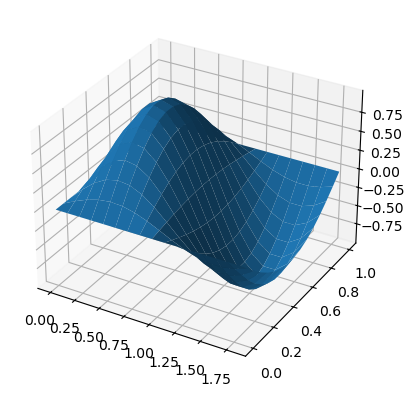
\includegraphics[width=0.3\textwidth]{src/1.png}
        \hspace{1cm}
        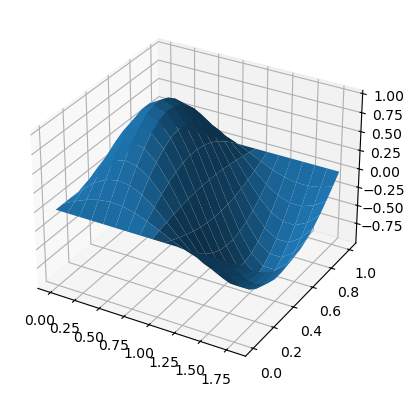
\includegraphics[width=0.3\textwidth]{src/2.png}
        \caption{Comparaison de la solution exacte et de la solution approchée pour $\mu = 1$}
        \label{fig:1}
    \end{figure}

    \newpage
    La différence en norme $L_2$ entre la solution exacte et la solution approchée est de $0.0539107877692071$. Notre implémentation est donc correcte.\\

    \item On prend maintenant en compte la condition de Neumann sur le bord $\Gamma_1$ :
    \begin{align*}
        \text{Soit } y \in [0, b] \quad u(a - h_x, y) &= u(a, y) - h_x \frac{\partial u}{\partial x}(a, y) + \frac{h_x^2}{2} \frac{\partial^2 u}{\partial x^2}(a, y) + \mathcal{O}(h_x^3) \\
        u(a - 2h_x, y) &= u(a, y) - 2h_x \frac{\partial u}{\partial x}(a, y) + 2h_x^2 \frac{\partial^2 u}{\partial x^2}(a, y) + \mathcal{O}(h_x^3) \\
        \Leftrightarrow \quad 4u(a - h_x, y) - u(a - 2h_x, y) &= 3u(a, y) - 2h_x \frac{\partial u}{\partial x}(a, y) + \mathcal{O}(h_x^3) \\
        \Leftrightarrow \quad \frac{\partial u}{\partial x}(a, y) &= \frac{3u(a, y) - 4u(a - h_x, y) + u(a - 2h_x, y)}{2h_x} + \mathcal{O}(h_x^2)
    \end{align*}

    \item La matrice $B$ est modifiée pour prendre en compte la condition de Neumann. On a alors : \\
    $B = \begin{pmatrix}
        1 & 0 & 0 & \dots & 0 \\
        -\frac{\mu}{h_x^2} & \frac{2\mu}{h_x^2} + \frac{2\mu}{h_y^2} & -\frac{\mu}{h_x^2} & \ddots & \vdots \\
        0 & \ddots & \ddots & \ddots & 0 \\
        \vdots & \ddots & -\frac{\mu}{h_x^2} & \frac{2\mu}{h_x^2} + \frac{2\mu}{h_y^2} & -\frac{\mu}{h_x^2} \\
        0 & \dots & \frac{1}{2h_x} & -\frac{4}{2h_x} & \frac{3}{2h_x}
    \end{pmatrix}$\\

\end{enumerate}

\section*{Approximation des termes advectifs}

\begin{enumerate}[resume]
    \item On introduit le nombre de Péclet $P_{e_l} = \frac{lv}{\mu}$, où $l$ est la longueur caractéristique du problème et $v$ la vitesse caractéristique. \\
    On suppose que $P_{e_l} \gg 1 \Leftrightarrow lv \gg \mu$ : le régime dominant est le régime advectif. \\

    \item On pose : $V = \begin{pmatrix}
        v_x \\
        0
        \end{pmatrix}$.
        En utilisant un développement limité à l'ordre 2 de $u(x_{i+1}, y_j)$ et de $u(x_{i-1}, y_j)$, on obtient :
        \begin{align*}
            u(x_{i+1}, y_j) &= u(x_i, y_j) + h_x \frac{\partial u}{\partial x}(x_i, y_j) + \frac{h_x^2}{2} \frac{\partial^2 u}{\partial x^2}(x_i, y_j) + \mathcal{O}(h_x^3) \\
            u(x_{i-1}, y_j) &= u(x_i, y_j) - h_x \frac{\partial u}{\partial x}(x_i, y_j) + \frac{h_x^2}{2} \frac{\partial^2 u}{\partial x^2}(x_i, y_j) + \mathcal{O}(h_x^3) \\
            \Leftrightarrow \quad \frac{\partial u}{\partial x}(x_i, y_j) &= \frac{u(x_{i+1}, y_j) - u(x_{i-1}, y_j)}{2h_x} + \mathcal{O}(h_x^2)\\
            \Leftrightarrow \quad V \cdot \nabla u(x_i, y_j) &= \begin{pmatrix}
                v_x \\
                0
            \end{pmatrix} \cdot
            \begin{pmatrix}
                \frac{\partial u}{\partial x}(x_i, y_j) \\
                \frac{\partial u}{\partial y}(x_i, y_j)
            \end{pmatrix}
        \end{align*}
        Donc : $V \cdot \nabla u(x_i, y_j) = v_x \frac{u(x_{i+1}, y_j) - u(x_{i-1}, y_j)}{2h_x} + \mathcal{O}(h_x^2)$.

        La matrice $A$ est modifiée pour prendre en compte les termes advectifs. On a alors : \\
        $A = \begin{pmatrix}
            I_d + D & 0 & 0 & \dots & 0 \\
            C & B & C & \ddots & \vdots \\
            0 & \ddots & \ddots & \ddots & 0 \\
            \vdots & \ddots & C & B & C \\
            0 & \dots & 0 & 0 & I_d + D \\
        \end{pmatrix} \quad \text{avec} \quad D = v_x \begin{pmatrix}
            0 & 0 & 0 & \dots & 0 \\
            \frac{1}{2h_x} & 0 & -\frac{1}{2h_x} & \ddots & \vdots \\
            0 & \ddots & \ddots & \ddots & 0 \\
            \vdots & \ddots & \frac{1}{2h_x} & 0 & -\frac{1}{2h_x} \\
            0 & \dots & 0 & 0 & 0
        \end{pmatrix}$\\

\end{enumerate}


\end{document}